\section{Schaltalgebra}
\subsection{Symbolik}
	Folgende Symbole werden verwendet:\\
	\begin{multicols}{4}
		$\neg=^-=$NOT
	\columnbreak
	
		$\vee=+=$OR
	\columnbreak
	
		$\wedge=*=$AND
	\columnbreak
	
		$\oplus=\$=$EXOR
	\end{multicols}
	
\subsection{Rechenregeln}
	\begin{tabular}{llll}
		Verkn"upfung mit 0 & $ a \vee 0 = a $ & $ a \wedge 0 = 0 $ & $ a \oplus 0 = a $\\
		Verkn"upfung mit 1 & $ a \vee 1 = 1 $ & $ a \wedge 1 = a $ & $ a \oplus 1 = \overline{a} $ \\
		Verkn. mit sich selbst & $ a \vee a = a $ & $ a \wedge a = a $ & $ a \oplus a = 0 $ \\
		Verkn. mit Inversem & $ a \vee \overline{a} = 1 $ & $ a \wedge \overline{a} = 0 $ & $ a \oplus \overline{a} = 1 $ \\
		\\
		Kommutativgesetz & $ a \vee b = b \vee a $ & $ a \wedge b = b \wedge a $ & $ a \oplus b = b \oplus a $\\
		Assioziativgesetz & $ (a \vee b) \vee c = a \vee (b \vee c) $ & $ (a \wedge b) \wedge c = a \wedge (b \wedge c) $ & $ (a \oplus b) \oplus c = a \oplus (b \oplus c) $ \\
		Distributivgesetz & $ a \wedge (b \vee c) = (a \wedge b) \vee (a \wedge c) $ & $ a \vee (b \wedge c) = (a \vee b) \wedge (a \vee c) $ & $ a \wedge (b \oplus c) = (a \wedge b) \oplus (a \wedge c) $ \\	
		\end{tabular}
		
\subsection{Vereinfachungen}
	\begin{multicols}{4}
		$ a \vee (a \wedge b) = a $ \\
		$ a \wedge (a \vee b) = a $ 
	\columnbreak
	
		$ (a \wedge \overline{b}) \vee b = a \vee b $ \\
		$ (a \vee \overline{b}) \wedge b = a \wedge b $ 
	\columnbreak
	
		$ (a \wedge \overline{b}) \oplus b = a \vee b $ \\
		$ (a \oplus \overline{b}) \wedge b = a \wedge b $ 
	\columnbreak
		
		$ (a \wedge b) \vee (a \wedge \overline{b}) = a $\\	
		$ (a \vee b) \wedge (a \vee \overline{b}) = a $
	\end{multicols}

\subsection{Shannon und DeMorgan}
	\begin{tabular}{lll}
		Ursprungsschaltung: & Shannon & DeMorgan\\
		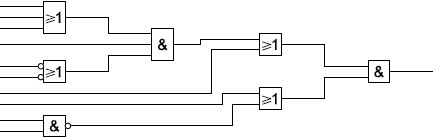
\includegraphics[width=0.3\textwidth]{pics/shanonursprung} & 
		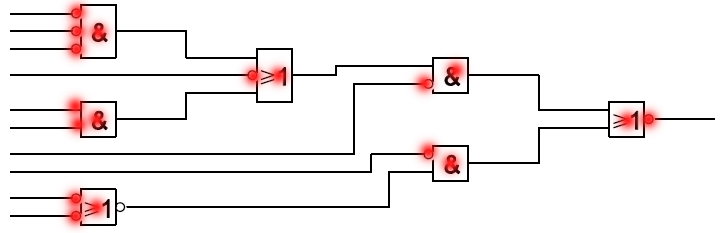
\includegraphics[width=0.3\textwidth]{pics/shanonende} &
		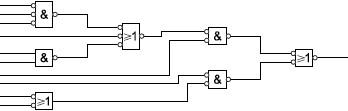
\includegraphics[width=0.3\textwidth]{pics/demorganende}\\
	\end{tabular}

\subsection{Normalformen}
	\begin{multicols}{3}
		Ausgangslage:\\
		\begin{tabular}{|l|l|l|l|l|}
			\hline	
				Dezimal & x2 & x1 & x0 & y \\	
			\hline
			\hline
				0 & 0 & 0 & 0 & 0 \\
			\hline	
				1 & 0 & 0 & 1 & 1 \\
			\hline
				2 & 0 & 1 & 0 & 0 \\
			\hline
				3 & 0 & 1 & 1 & 1 \\
			\hline
				4 & 1 & 0 & 0 & 0 \\
			\hline
				5 & 1 & 0 & 1 & d \\
			\hline
				6 & 1 & 1 & 0 & 1 \\
			\hline
				7 & 1 & 1 & 1 & 1 \\
			\hline
		\end{tabular}
		\columnbreak
		
		\subsubsection{Kanonisch disjunktive Normalform}
			\begin{tabular}{|l|}
				\hline
				\\
				\hline
					$\overline{x2} \wedge \overline{x1} \wedge x0$ \\
				\hline
				\\
				\hline
					$\overline{x2} \wedge x1 \wedge x0$ \\
				\hline
				\\
				\hline
					$[x2 \wedge \overline{x1} \wedge x0]$ \\
				\hline
					$x2 \wedge x1 \wedge \overline{x0}$ \\
				\hline
					$x2 \wedge x1 \wedge x0$ \\
				\hline	
			\end{tabular}
			$y=(\overline{x2} \wedge \overline{x1} \wedge x0) \vee (\overline{x2} \wedge x1 \wedge x0) \vee [x2 \wedge \overline{x1} \wedge x0] \vee (x2 \wedge x1 \wedge \overline{x0}) \vee (x2 \wedge x1 \wedge x0)$ \\
			Es werden nur diejenigen Zeilen der Wahrheitstabelle aufgef"uhrt, deren Funktionswert 1 oder d ist.
		\columnbreak
				
		\subsubsection{Kanonisch konjunktive Normalform}
			\begin{tabular}{|l|}
				\hline
					$x2 \vee x1 \vee x0$ \\
				\hline
				\\
				\hline
					$x2 \vee \overline{x1} \vee x0$ \\
				\hline
				\\
				\hline
					$\overline{x2} \vee x1 \vee x0$ \\
				\hline
					$[\overline{x2} \vee x1 \vee \overline{x0}]$ \\
				\hline
				\\
				\hline
				\\
				\hline	
			\end{tabular}
			$y=(x2 \vee x1 \vee x0) \wedge (x2 \vee \overline{x1} \vee x0) \wedge (\overline{x2} \vee x1 \vee x0) \wedge [\overline{x2} \vee x1 \vee \overline{x0}]$ \\
			Es werden nur diejenigen Zeilen der Wahrheitstabelle aufgef"uhrt, deren Funktionswert 0 oder d ist.
	\end{multicols}

\subsection{Karnaugh-Diagramm}
	\begin{multicols}{3}
		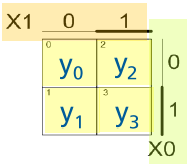
\includegraphics[width=0.3\textwidth]{pics/kv/2erKV} 
	\columnbreak
	
		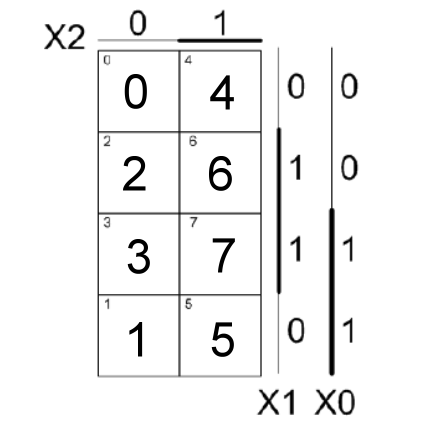
\includegraphics[width=0.3\textwidth]{pics/kv/3erKV}
	\columnbreak
	
		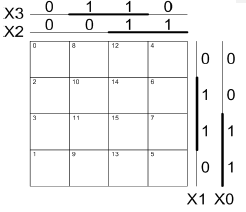
\includegraphics[width=0.3\textwidth]{pics/kv/4erKV}
	\end{multicols}
	
	\subsubsection{Arbeiten mit dem KV-Diagramm}
		\begin{compactitem}
			\item 1) \ \ Aufstellen der Wahrheitstabelle.\\
			\item 2) \ \ "Ubertragen der Werte der Wahrheitstabelle in KV Diagramm.\\
			\item 3) \ \ M"oglichst grosse Gruppen a $2^n$ Felder bilden.\\
			\item 4)
				\begin{tabular}{ll}
					Kanonisch disjunktive Normalform: & Kanonisch konjunktive Normalform: \\
					Gruppen von Feldern mit Wert 1 oder d & Gruppen von Feldern mit Wert 0 oder d\\
					Primimplikanten: AND Verkn"upfung & Primimplikanten: OR Verkn"upfung\\
					OR Verkn"upfung aller Primimplikanten & AND Verkn"upfung aller Primimplikanten\\
				\end{tabular}
		\end{compactitem}